\paragraph[QuizziPedia::Front-End::Controllers\\::FillingQuestionnaireController]{QuizziPedia::Front-End::Controllers::FillingQuestionnaireController}
\begin{figure} [ht]
	\centering
	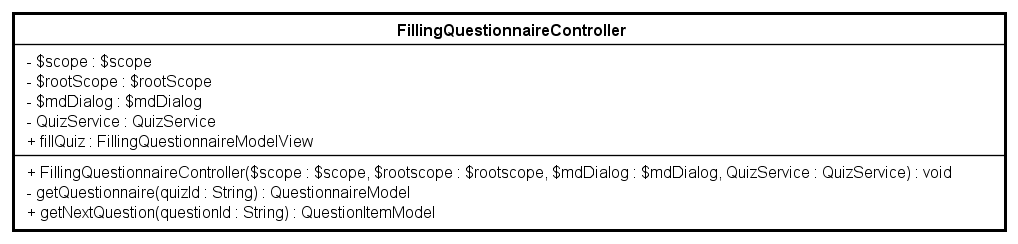
\includegraphics[scale=0.45]{UML/Classi/Front-End/QuizziPedia_Front-end_Controller_FillingQuestionnaireController.png}
	\caption{QuizziPedia::Front-End::Controllers::FillingQuestionnaireController}
\end{figure} \FloatBarrier
\begin{itemize}
	\item \textbf{Descrizione}: questa classe permette di gestire la compilazione del questionario;
	\item \textbf{Utilizzo}: fornisce le funzionalità per compilare un questionario e per gestire il cambio di domanda;
	\item \textbf{Relazione con altre classi}:
	\begin{itemize}
		\item \textbf{IN} \texttt{FillingQuestionnaireModelView}: classe di tipo modelview la cui istanziazione è contenuta all'interno della variabile di ambiente \$scope di \textit{Angular\ped{G}}. All'interno di essa sono presenti le variabili e i metodi necessari per il \textit{Two-Way Data-Binding\ped{G}} tra la \textit{view\ped{G}} \texttt{FillingQuestionnaireView} e il \textit{controller\ped{G}} \texttt{FillingQuestionnaireController};  
		\item \textbf{IN} \texttt{InfoQuestionnaireTemplate}: rappresenta il componente grafico che permette all'utente di visualizzare le informazioni principali del questionario che si sta per svolgere. Viene gestito dinamicamente all'interno della \textit{view\ped{G}} \texttt{TrainingView} attraverso il \textit{controller\ped{G}} \texttt{TrainingController};
		\item \textbf{IN} \texttt{QuizService}: permette di ottenere i dati di un quiz tramite delle parole chiave inserite dall'utente nella barra di ricerca. Permette inoltre di iscriversi ad un questionario e di scaricare l'intera lista di domande di un questionario a partire dal suo id univoco;
		\item \textbf{IN} \texttt{QuestionnaireModel}: rappresenta un questionario. Contiene tutte le informazioni necessarie alla presentazione del contenuto del questionario;
		\item \textbf{IN} \texttt{QuestionsController}: questa classe permette di gestire il recupero delle domande per far si che possano essere visualizzate nella modalità allenamento e nella compilazione dei questionari; 
		\item \textbf{IN} \texttt{QuestionItemModel}: rappresenta una domanda. Contiene tutte le informazioni necessarie alla presentazione del contenuto della domanda.
	\end{itemize}
	\item \textbf{Attributi}:
	\begin{itemize}
		\item \texttt{-} \texttt{\$scope: \$scope} \\
		Campo dati contenente un riferimento all'oggetto \$scope creato da \textit{Angular\ped{G}}, viene utilizzato come mezzo di comunicazione tra il \textit{controller\ped{G}} e la \textit{view\ped{G}}. Contiene gli oggetti che definiscono il \textit{model\ped{G}} dell'applicazione;
		\item \texttt{-} \texttt{\$rootScope: \$rootScope} \\
		Campo dati contenente il riferimento all'oggetto globale \$rootScope creato da \textit{Angular\ped{G}}. Viene utilizzato per rendere accessibile a tutti i \textit{controller\ped{G}} e a tutte le \textit{view\ped{G}} l'oggetto \texttt{QuestionnaireModel}. In questo caso viene utilizzato per inserire in \$rootScope l'oggetto di ritorno della chiamata a \texttt{getNextQuestion} e l'intero questionario ritornato dalla chiamata a \texttt{getQuestionnaire};
		\item \texttt{-} \texttt{\$mdDialog: \$mdDialog} \\
		Campo dati contenente un riferimento al servizio della libreria \textit{Material for Angular\ped{G}} che permette di creare delle componenti a pop-up;
		\item \texttt{-} \texttt{QuizService: QuizService}: questa classe permette di ottenere i dati di un quiz tramite delle parole chiave inserite dall'utente nella barra di ricerca. Permette inoltre di iscriversi ad un questionario e di scaricare l'intera lista di domande di un questionario a partire dal suo id univoco;
		\item \texttt{+} \texttt{fillQuiz: FillingQuestionnaireModelView} \\
		Oggetto di tipo \texttt{FillingQuestionnaireModelView}. All'interno di esso sono presenti le variabili e i metodi necessari per il \textit{Two-Way Data-Binding\ped{G}} tra la \textit{view\ped{G}} \texttt{FillingQuestionnaireView} e il \textit{controller\ped{G}} \texttt{FillingQuestionnaireController};
		\item \locationA;
		\item \routeparamsA;
		\item \errorinfomodelA;
		\item \questionnairemodelA;
		\item \timeoutA;
		\item \texttt{-} \texttt{quizIsLoaded: Boolean} \\ Campo dati che indica se il questionario è stato scaricato;
		\item \texttt{-} \texttt{questionNumberOnQuiz: Number} \\ Campo dati che indica il numero progressivo della domanda mostrata;
		\item \texttt{-} \texttt{startQuiz: Boolean} \\ Campo dati che indica se il questionario è pronto per essere iniziato;
		\item \texttt{-} \texttt{noStart: Boolean} \\ Campo dati che indica se il questionario è abilitato alla compilazione;
		\item \texttt{-} \texttt{started: Boolean} \\ Campo dati che indica se il questionario è stato iniziato;
		\item \texttt{-} \texttt{quizIsFinished: Boolean} \\ Campo dati che indica se il questionario è finito;
		\item \texttt{-} \texttt{noAuth: Boolean} \\ Campo dati che indica se l'utente che si posiziona nel questionario ha o meno l'autorizzazione;
		\item \texttt{-} \texttt{questions: Array<QuestionItemModel>} \\ Campo dati che rappresenta le domande che verranno poste all'utente;
		\item \texttt{-} \texttt{quiz: QuestionnaireModel} \\ Campo dati che rappresenta il questionario;
		\item \texttt{-} \texttt{myChartDataDoughnut: Object} \\ Campo dati che rappresenta i dati che verranno mostrati nel grafico finale;
		\item \texttt{-} \texttt{myChartOptionsDoughnut: Object} \\ Campo dati che rappresenta le opzioni per la rappresentazione del grafico finale.
	\end{itemize}
	\item \textbf{Metodi}:
	\begin{itemize}
		\item \texttt{+} \texttt{FillingQuestionnaireController(\$scope: \$scope, \$rootScope: \$rootScope, \$mdDialog: \$mdDialog, QuizService: QuizService, \$timeout:\$timeout, \$location:\$location, \$routeParams: \$routeParams, ErrorInfoModel: ErrorInfoModel, QuestionnaireModel: QuestionnaireModel)} \\Metodo costruttore della classe.\\
		\textbf{Parametri}:
		\begin{itemize}
			\item \texttt{\$scope: \$scope} \\
			Parametro contenente un riferimento all'oggetto \$scope creato da \textit{Angular\ped{G}}. Viene utilizzato come mezzo di comunicazione tra il \textit{controller\ped{G}} e la \textit{view\ped{G}}. Contiene gli oggetti che definiscono il viewmodel e il \textit{model\ped{G}} dell'applicazione;
			\item \texttt{-} \texttt{\$location: \$location} \\
			Parametro contenente un riferimento al servizio creato da \textit{Angular\ped{G}} che permette di accedere alla barra degli indirizzi del \textit{browser\ped{G}}, i cambiamenti all’URL nella barra degli indirizzi si riflettono in questo oggetto e viceversa;
			\item \texttt{\$mdDialog: \$mdDialog} \\
			Parametro contenente un riferimento al servizio della libreria \textit{Material for Angular\ped{G}} che permette di creare delle componenti a pop-up;
			\item \texttt{QuizService: QuizService}:\\ Parametro che permette di ottenere, tramite il service, la lista di tutte le domande presenti nel quiz;
			\item \locationP;
			\item \routeparamsP;
			\item \errorinfomodelP;
			\item \questionnairemodelP;
			\item \timeoutP.
		\end{itemize}
		\item \texttt{-} \texttt{downloadQuiz(): void}: \\ Metodo che ottiene l'intero questionario; \\
		\item \texttt{+} \texttt{nextQuestion(): void}: \\ Metodo che carica la domanda successiva del quiz tramite chiamata a \texttt{QuestionController}; \\
		\item \texttt{+} \texttt{startQuizClick(): void} \\
		Metodo che gestisce l'evento per iniziare il questionario;
		\item \texttt{+} \texttt{endQuiz(): void} \\
		Metodo che gestisce l'evento per terminare il questionario in modo anticipato;
		\item \texttt{+} \texttt{goToHome(): void} \\
		Metodo che gestisce l'evento per tornare alla pagina principale dell'applicazione;  
		\item \texttt{+} \texttt{\$on('\$locationChangeStart': String, callback: function): void} \\
		Metodo che gestisce l'evento per tornare alla pagina principale dell'applicazione.\\
		\textbf{Parametri}:
		\begin{itemize}
			  	\item \texttt{-} \texttt{'\$locationChangeStart': String} \\
			  	Parametro che indica su quale evento rimanere in ascolto;
			  	\item \texttt{-} \texttt{callback: function} \\
			  	Parametro che indica una funzione da eseguire.
		\end{itemize}
		\item \texttt{+} \texttt{\$on('addResult', callback: function): void} \\
		Metodo che gestisce l'evento per aggiornare i risultati dati alle domande. \\
		\textbf{Parametri}:
		\begin{itemize}
			\item \texttt{-} \texttt{'addResult': String} \\
			Parametro che indica su quale evento rimanere in ascolto;
			\item \texttt{-} \texttt{callback: function} \\
			Parametro che indica una funzione da eseguire.
		\end{itemize}
		\item \texttt{+} \texttt{graphResultAfterFinishedATraining(): void} \\
		Metodo imposta le variabili per la visualizzazione del grafico finale. 
	\end{itemize}
\end{itemize}

